\scanpage{100}\mspage{96}
composition est associative, avec \deleted{\unsure{les|des}}\inserted{\unsure{comme|pour}} identités $\deleted{\unsure{\mathrm{id}_{\underline E}|\alpha_{\underline E}}}\sigma_{\underline E}=\operatorname{supp}^{\unsure{\circ|\bullet}}_{\underline E}\circ\mathrm{id}_{\unsure{E|\underline E}}$. La catégorie des \unsure{disjoncteurs|disponcteurs|disponteurs} et correspondances \deleted{\unsure{de|des}}\inserted{entre} \unsure{telles|icelles|elles}, est \unsure{équivalente} à la catégorie des disjoncteurs canoniques ou \unsure{spatios} (ou ``\uline{\unsure{espaceurs}}'' ?), \unsure{ou|où} on prend comme morphismes les \uline{applications} \unsure{croissantes} qui commutent aux sup quelconques\inserted{(appelées encore ``correspondances'' entre les spatios)}. Et cette catégorie est canoniquement équivalente à la catégorie opposée, par une ``autodualité'' (involutive) qui est l'identité sur les objets, et sur les morphismes est le passage à la \unsure{flèche|flèches} transposée\unsure{.|..}

[Analogie avec les espaces de Hilbert, ou \inserted{plus \unsure{gén.|gén}} espaces vectoriels munis d'une autodualité\ldots, et les opérateurs adjoints\ldots]

\margin{\figure{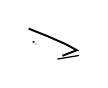
\begin{tikzpicture}[x=1em,y=1em]
 \draw[line width=.7pt] (0,1.1) -- (.7,.82) -- (1.36,.53) -- (1.74,.32) -- (1.22,.12);
 \draw[line width=.45pt] (1.04,0) -- (1.82,.13);
 \fill (.18,.62) ellipse (.055 and .03);
 \fill (.27,.54) circle (.022);
\end{tikzpicture}}}\uline{Questions ouvertes}, que je ne vois pas moyen de tirer au clair, \unsure{suggérées} par le cas des disjoncteurs triviaux.
% archive sheet number: 99
